
%NOTE: to be used with \usepackage{subfiles} in the main file.
%Subfiles go in folders which live with the main file.
%Bibliography and preamble go in the main file.

%%%%%%%%%%%%%%%%%%%%%%%% PREAMBLE %%%%%%%%%%%%%%%%%%%%%%%%

\providecommand{\main}{..}

\documentclass[main]{subfiles} %Each instance of `../' elevates one folder to find the main file

\begin{document}

%%%%%%%%%%%%%%%%%%%%%%% DOCUMENT %%%%%%%%%%%%%%%%%%%%%%%

% \tableofcontents % Can be useful to load a TOC while writing

\doublespacing

\schapter{Theoretical aspects}

\hypsection{Jets and algorithms}
\vspace{20pt}
After being produced in a high-energy event, quarks and gluons fragment and hadronize resulting in a collimated spray of hadrons called a jet. The reason behind the process of hadronization lies in the concept of colour confinement. In quantum chromodynamics (QCD), colour confinement states that only objects with non zero colour charge can propagate as free particles, therefore quarks and gluons are only seen bound together in the form of hadrons. When particles carrying colour charge (namely quarks and gluons) are separated in a high-energy event, new colour carrying particles are spontaneously created from the vacuum in order to form colourless hadrons, thus obeying confinement. \\

While hadronization is not yet fully understood and a theoretical description of the process is not yet available, there is a number of phenomenological models such as the Lund String Model that do a good job of describing it \cite{Andersson1983}. The phenomenon can be understood qualitatively through these models by taking into account that the gluon field between colour charges becomes a narrow flux tube as they get separated and eventually it becomes energetically favourable for a new particle to appear rather than extending the tube further, as can be seen in figure \ref{fig:hadronization}.\\

\begin{figure}[h]
    \centering
    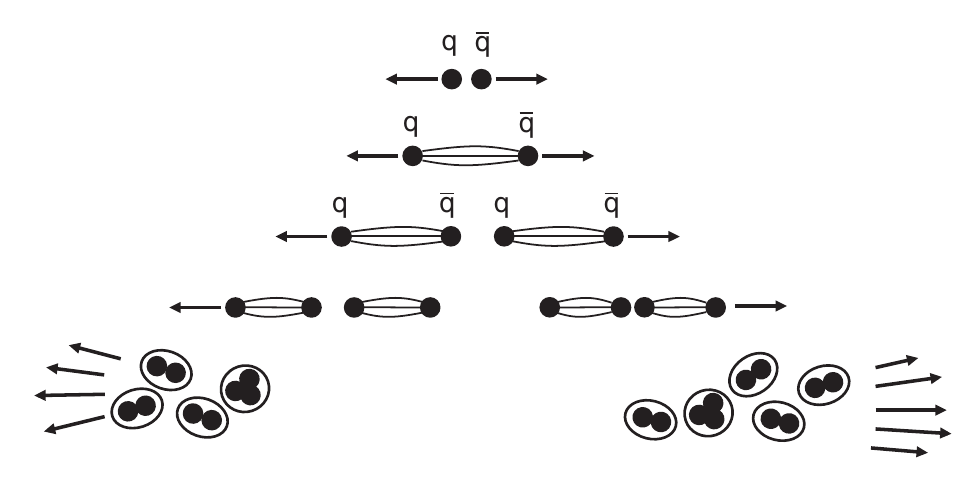
\includegraphics[width=0.8\textwidth]{../Figures/Theory/hadronization.png}
    \caption{Schematic representation of the hadronization process. Picture taken from \cite{Thomson2013}.}
    \label{fig:hadronization}
\end{figure}

The particles resulting from the hadronization of a single quark (parton) tend to travel in the same direction as their parent forming a narrow cone, which is what is known as a jet. In particle detector experiments jets are observed instead of quarks, and their structure is quite visible when looking at the events reconstructed in the detector. Through the measurement of the different properties of a jet it is possible to obtain information about the original parton that originated it. Therefore jets are an essential part of the analyses carried out in collider experiments.\\

As important as they are, to be used effectively in analyses jets need to be well defined. As stated in the work of \citet{Salam2010} a jet definition is constituted by a jet algorithm with its respective parameters and recombination scheme. A jet algorithm is a set of rules that group particles into jets. These algorithms usually involve parameters that govern their behaviour, for example in defining how close two particles need to be in order for them to be considered part of the same jet. Jet algorithms are also related to a certain recombination scheme, which indicates how the momentum is assigned to the object resulting of merging two particles during a clustering process.\\

Jet algorithms can be usually classified into two broad categories: cone algorithms and sequential recombination algorithms. Cone algorithms originate from the initial idea of \citet{Sterman1977}. They are considered "top-down" algorithms, since they group together particles within specific conical angular regions so that the resulting cone is "stable", meaning that the direction of the cone matches that of the 4-momenta sum of the particles. On the other hand, sequential recombination algorithms are considered "bottom-up", as they iteratively recombine nearby particles in accordance to a certain distance measure.\\

The anti-$k_t$ algorithm \cite{Cacciari2008} is a sequential recombination algorithm widely used in collider experiments, being also the preferred jet identification algorithm in ATLAS analyses. Since the present study is based on simulated data from this detector (see section \ref{sect:event-generation-chain}) it is relevant to give a brief overview of this algorithm. The anti-$k_t$ takes as an input a list of $N$ objects and it returns a list of jets, which correspond to clusters of said objects grouped according to specific rules regarding distances between them. The distances used by the algorithm are calculated from the quantities $k_{tX}$, $\eta_X$ and $\phi_X$ which correspond to the transverse momentum, pseudo-rapidity and azimuthal angle of the object $X$. These distances are $d_{ij}$ (the distance between objects $i$ and $j$) and $d_{iB}$ (the distance between the object $i$ and the beam), they are defined as follows:
\begin{align}
  d_{ij} &= \text{min}(k_{ti}^{-2},k_{tj}^{-2})\frac{\Delta_{ij}^2}{R^2}\\
  d_{iB} &= k_{ti}^{-2}
\end{align}
where $\Delta_{ij}^2 = (\eta_i - \eta_j)^2 + (\phi_i - \phi_j)^2$ and $R$ is the radius parameter that sets the size scale of the jets found. The algorithm iteratively forms clusters by identifying the smallest of the two distances for all the objects in the input list. If $d_{ij}$ is the smallest, objects $i$ and $j$ are recombined and replaced in the object list by the recombined object. If on the other hand $d_{iB}$ is the smallest, object $i$ is removed from the object list and marked as a jet.\\


\hypsection{The LHC and the ATLAS detector}
\vspace{15pt}
The Large Hadron Collider (LHC) is \dots

\hypsection{Boosted objects and fat jets}
\vspace{15pt}

\hypsection{Jet tagging}
\vspace{15pt}

\hypsection{Fat jet substructure: Nsubjettiness}
\vspace{15pt}

\hypsection{TMVA Classifiers}
\vspace{15pt}

\hypsection{Event generators}
\vspace{15pt}



















% \bibliographystyle{../../PhilReview} %%bib style found in bst folder, in bibtex folder, in texmf folder.
% \nobibliography{Zotero} %%bib database found in bib folder, in bibtex folder
% \nobibliography{../../Thesis_bib}
\biblio

\end{document}
